


\paragraph{Relative Time Protocol:}

The elected validators for a slot need to know when the right time is to produce a block for the consistency and the security of BABE. For this, validators uses their local computer clock which is not adjusted by  any centralized clock adjustment protocols such as the Network Time Protocol \cite{ntp}. Instead, they keep their clock synchronised with the other validators with the relative time protocol. 
% \eray{when actually the right time to produce a block for the consistency and the security of the block production mechanism}{-comment:This sentence does not have a verb-}.
%For this purpose, they run the relative time protocol which lets them know when approximately a slot starts even if some clock drifts exist in their local clock. We note that in BABE, we do not rely on any centralized clock adjustment protocols such as the Network Time Protocol \cite{ntp}. 
%Therefore, we design the relative time protocol that depends on the arrival time of blocks according to local clocks of validators. 
%\eray{``Relative Time''}{``relative time protocol"}.
The formal security model of local clock synchronisation in blockchains without NTP and further details about the relative time protocol can be found in \cite{consensusonclock}.
%\eray{Please see \cite{consensusonclock} for the formal security model of synchronization in blockchains and for further details about the relative time protocol.}{The formal security model of synchronization in blockchains and further details about the relative time protocol can be found in \cite{consensusonclock}.}

In BABE, we assume that after the genesis block is released, elected validators of the first epoch store the arrival time of the genesis block with respect to their local clock. Then, they mark the beginning
 time of the first slot and increment
the slot number every $ T $ seconds. After this point,  they periodically run the relative algorithm not to lose the synchronisation with others because of their local clock drifts.  In addition to this, a validator who
joins after the genesis block runs the relative time algorithm to be synchronised with the other validators.

In every sync-epochs (different than epochs in BABE), validators update their clock according to the result of the relative time protocol and use the new clock until the next sync-epoch. The first sync-epoch $\varepsilon_1$ starts just after the genesis block is released. The other sync-epochs  $\varepsilon_i$ start when the slot number of the last (probabilistically) finalised block is $\bar{sl}_{\epsilon}$ which is the smallest slot number such that  $\bar{sl}_{\varepsilon} - \bar{sl}_{\varepsilon-1} \geq s_{cd}$ where $\bar{sl}_{\varepsilon-1}$ is the slot number of the last (probabilistically) finalized block in sync-epoch $\varepsilon-1$. Here, $s_{cd}$ is the parameter of the chain density (CD) property which will be defined according the chain growth.
In more detail, each validator  stores  the arrival time $ t_j $ of  blocks together with the slot number $\slot'_j$ in the block during a sync-epoch. At the end of a sync-epoch, the validator retrieves the arrival time of probabilistically finalized blocks generated during the sync-epoch and computes some candidate start times of the first slot $ \slot $ of the next sync-epoch i.e,  given that $ a_j = T(\slot - \slot'_j)  $,  $\mathcal{C}_T = \{t_j+a_j \}$. The times in $ \mathcal{C}_T $ are considered as candidates. In order to  choose one candidate,  the validator then sorts the list of candidates $ \mathcal{C}_T $ and outputs the median of the sorted list as a start time of the $ \slot $. An example execution of the relative time protocol in the first sync-epoch is in Figure \ref{fig:relativetime}.

\begin{figure}[h]
	\centering
	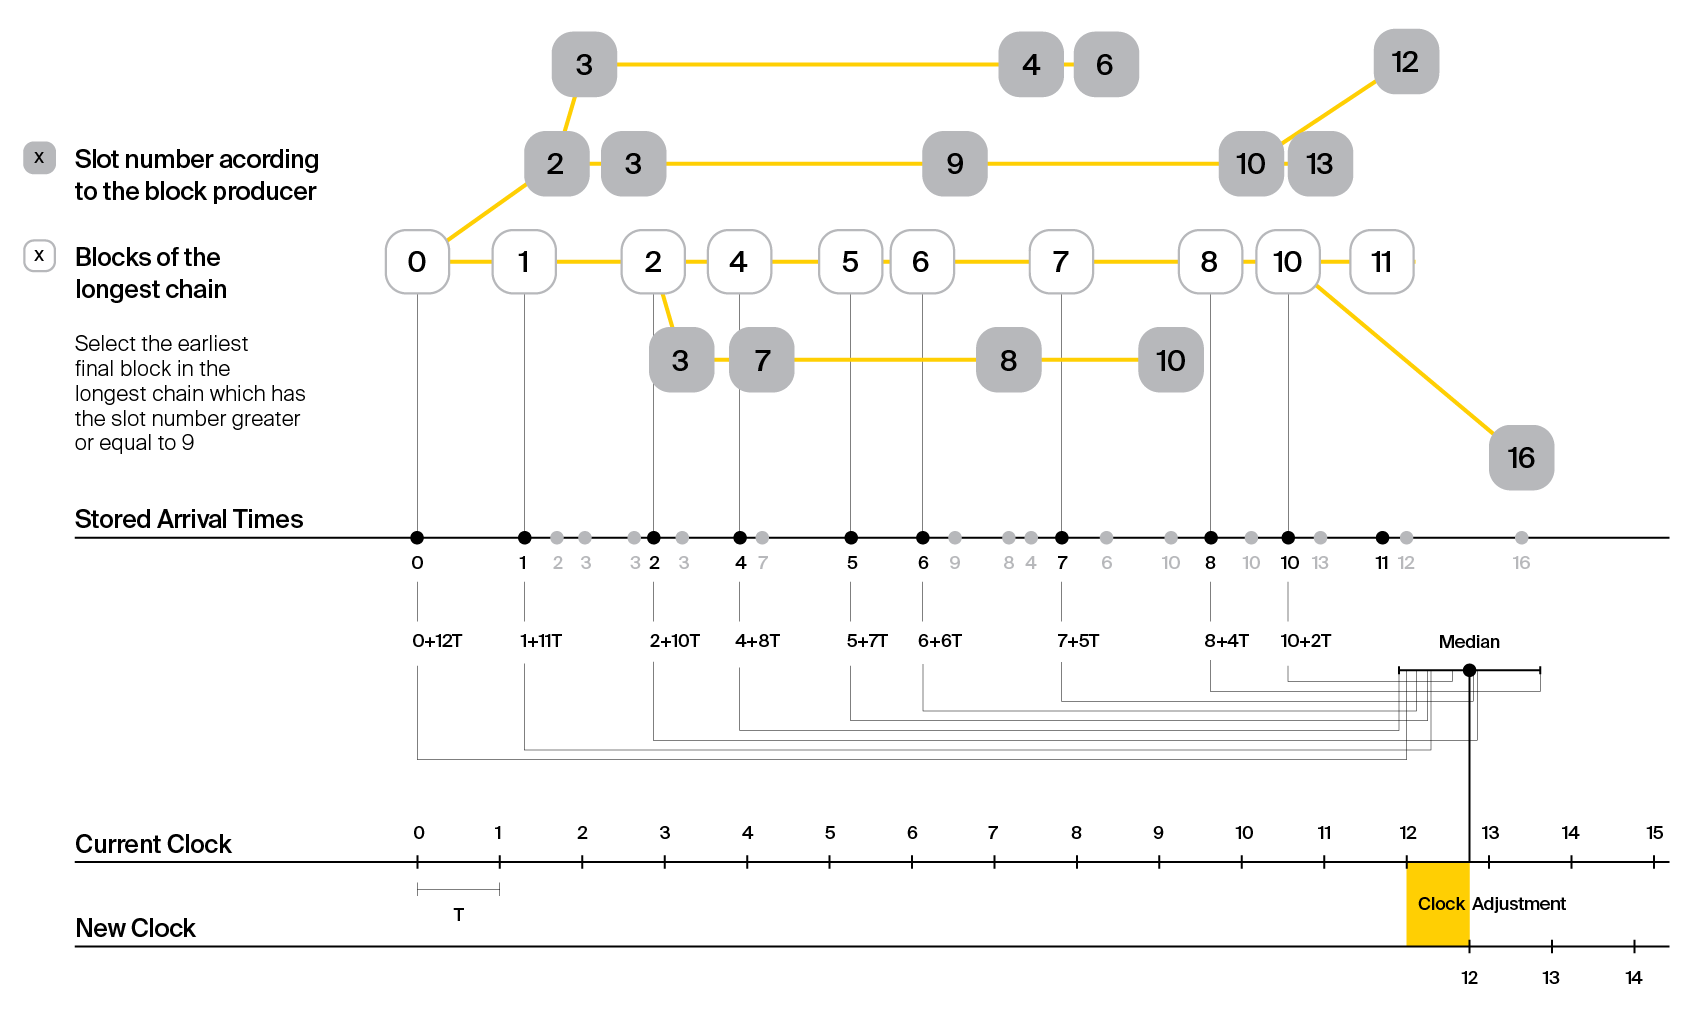
\includegraphics[width=1.\textwidth]{images/BABE3.png}
	\caption{An example execution of the relative time protocol in the first epoch where $s_{cd} = 9$ (image credit: Ignasi Albero).}
	\label{fig:relativetime}
\end{figure}
